\documentclass[../momento_1.tex]{subfiles}

\begin{document}

A terceira fase foi necessário acrescentar a implementação do grupo \textit{unpredictableTable} da \textit{Unpredictable MIB}. Considerámos que  os valores N=T, D=K e p=q=1 e são constantes. Não foi pedido ainda a implementação da operação de refrescamento da tabela de números aleatórios nem a operação de \textit{reset}, ou seja, a tabela construída no arranque do agente a partir da matriz $M_{t,k}$ do ficheiro de sementes foi mantida fixa e constante.\par 

Para a conceção do que era requerido no enunciado do projeto para esta fase, foi necessário primeiramente aceder e ler o ficheiro que contém as \textit{seeds}, como podemos ver no Exemplo  \ref{lst:seeds}, cuja diretoria foi obtida através do ficheiro de configuração previamente lido.\\ 

{\setstretch{1.1}
\begin{lstlisting}[caption={Método utilizado para obtenção das \textit{seeds}.},label={lst:seeds},language=JAVA]
	private void getSeeds() throws IOException {
        File conf = new File(seedPat);
        if (conf.exists()) { // if exists it's true
            BufferedReader fileParameters;
            String param;
            fileParameters = new BufferedReader(new FileReader("1st-seed"));
            while ((param = fileParameters.readLine()) != null) {
                seeds.add(param);
            }
        } else {
            System.out.println("Sem ficheiro de configuracao.\nColoque na pasta respectiva!");
            System.out.println("Pasta  " + System.getProperty("user.dir"));
            System.exit(0);
        }
    }
\end{lstlisting}}

Com os valores das \textit{seeds} armazenados pelo sistema, iniciámos a implementação da obtenção da matriz de números aleatórios. Como os valores dos parâmetros eram constantes, levando assim a que a matriz resultante fosse igual a $M_{t,k}$, desenvolvemos o método do Exemplo \ref{lst:matriz}, que dos valores das \textit{seeds} armazenados constrói a matriz resultante, no nosso caso de 8 colunas e 256 linhas.\\[1cm]

{\setstretch{1.1}
\begin{lstlisting}[caption={Método utilizado para obtenção da matriz de números aleatórios.},label={lst:matriz},language=JAVA]
	private char[][] getMatrix() {
        int numSize = Integer.parseInt(numberSize);
        int tabSize = Integer.parseInt(tableSize);
        char[][] matriz = new char[tabSize][numSize];
        for (int i = 0; i < tabSize; i++) {
            String aux = seeds.get(i);
            for (int j = 0; j < numSize; j++) {
                char[] split = aux.toCharArray();
                matriz[i][j] = split[j];
            }
        }
        return matriz;
    }
\end{lstlisting}}

Após a execução do método e respetiva obtenção da matriz, de seguida foi necessário guardar os valores correspondentes na MIB, mais propriamente na \textit{unpredictableTable}. Para que isto fosse possível implementámos o método do Exemplo \ref{lst:set}. Este método cria uma nova linha na tabela da MIB para cada linha da matriz original guardando o seu valor. É feita também a correspondência entre os valores guardados e uma chave na tabela, criando um novo OID para cada linha para que depois estes possam ser obtidos pela comando \textit{snmpget}.\\

{\setstretch{1.1}
\begin{lstlisting}[caption={Método utilizado para guardar a matriz na tabela da MIB.},label={lst:set},language=JAVA]
	private void setValue(Object value) {
        DefaultMOMutableTableModel model = (DefaultMOMutableTableModel) uminhogrmib.getRandomEntry().getModel();
        Variable[] v = new Variable[]{getOctetString(value)};
        model.addRow(model.createRow((new OID(new int[]{i})), v));
        i++;
    }
\end{lstlisting}}

Depois da implementação estar concluída o grupo iniciou a fase de testes ao sistema desenvolvido até  ao momento. Os testes elaborados consistiram na execução o agente e posterior obtenção dos valores da tabela através do comando \textit{snmpget} como podemos visualizar na Figura \ref{fig:faseC}.\\ 

\begin{figure}[H]
\centering
\captionsetup{justification=centering,margin=2cm}
\centerline{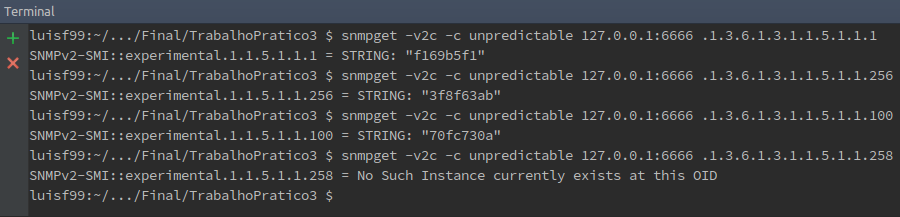
\includegraphics[scale=0.4]{../imagens/faseC.png}}
\caption{Teste realizados ao sistema na fase B.}
\label{fig:faseC}
\end{figure}

Como se pode verificar na figura e através da consulta dos valores presentes no ficheiro que contém as \textit{seeds}, os valores correspondem comprovando assim que o serviço implementado funciona sem quaisquer problemas.\\[17cm]


\end{document}
